Natural Language Processing (NLP) is a sub-field of Artificial Intelligence (AI) that deals with the understanding and generation of natural human languages.

Recently many of the tasks traditionally addressed by statistical NLP methods have been moving towards the adoption of neural networks to parameterize more expressive models of language. This includes tasks like machine translation, dialogue modelling, abstract summarization, document classification, etc.

In this thesis, we address the problem of neural disentanglement of style and content in text. We build a unified model that learns separately regularized latent spaces, thereby isolating both style and content. The main benefit of doing this is that the separate latent representations are now interpretable on a macro-level with respect to the style, as we control the flow of style-related information in the model.

As an added benefit, this disentangling model can also be directly applied to the problem of text style transfer. This is analogous to style transfer in computer vision \citep{gatys2016image}. The requirement of the style transfer task in the vision domain is to transfer the visual style from one image to the other, as illustrated in Figure \ref{fig:style-transfer-vision}. Stylistic transfer in text is based on a similar premise, wherein, given an arbitrary body of text and a predefined style - governed by a set of one or more attributes like sentiment, emotion, tense, authorship, etc. - a new body of text can be generated such that it incorporates the predefined style its generation is being conditioned on. We evaluate the efficacy of our method by generating text conditioned on any of a given set of discrete `labels' (used interchangeably with `attribute' or `style' henceforth).

\begin{figure}[ht]
	\centering
	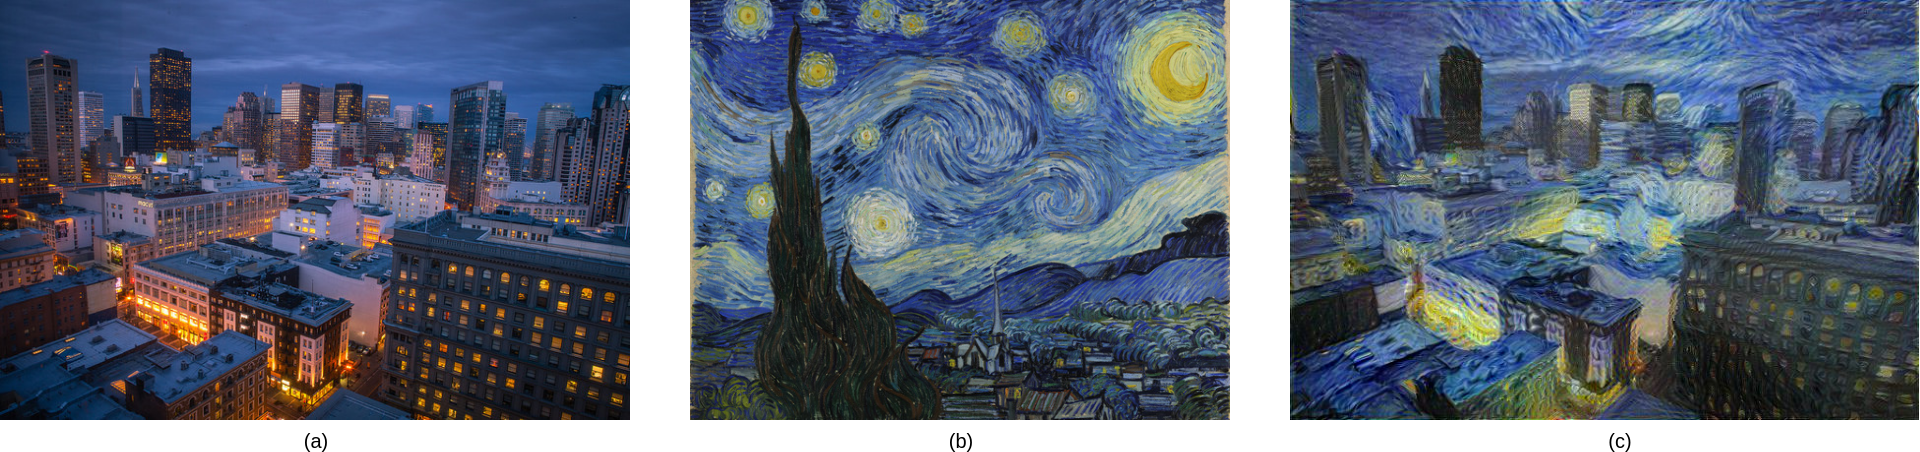
\includegraphics[width=\textwidth]{images/style-transfer-vision}
	\imgsrc{\url{https://github.com/fzliu/style-transfer}}
	\caption{\label{fig:style-transfer-vision}Visual Style Transfer: (a) Content, (b) Style and (c) Synthesized Images}
\end{figure}


\begin{table}[ht]
	\centering
	\begin{tabular}{ | p{.45\linewidth} | p{.45\linewidth} | }
		\hline
		\tabc{1}{Input}                                             & \tabh{Output}                                        \\
		\hline \hline
		i will bite thee by the ear for that jest .                 & i ’ ll bite you by the ear for that joke .           \\
		\hline
		what further woe conspires against mine age ?               & what ’ s true despair conspires against my old age ? \\
		\hline
		how doth my lady ?                                          & how is my lady ?                                     \\
		\hline
		hast thou slain tybalt ?                                    & have you killed tybalt ?                             \\
		\hline
		an i might live to see thee married once , i have my wish . & if i could live to see you married, i ’ ve my wish . \\
		\hline
		benvolio , who began this bloody fray ?                     & benvolio , who started this bloody fight itself ?    \\
		\hline
		what is your will ?                                         & what do you want ?                                   \\
		\hline
		call her forth to me .                                      & bring her out to me .                                \\
		\hline
	\end{tabular}
	\imgsrc{\cite{xu2012paraphrasing}}
	\caption{Authorship Style Transfer from Shakespearean Plays}
	\label{tab:paraphrasing-for-style-results}
\end{table}

The task of style transfer in context of text was first introduced by \cite{xu2012paraphrasing} as a statistical model that attempted to paraphrase bodies of text in a different style using a simple phrase replacement strategy. A few examples from this paper are shown in Table \ref{tab:paraphrasing-for-style-results}. Although fairly crude, this retrieve and replacement strategy is effective, given a large dataset with enough phrase context overlap. Since the overwhelming adoption of neural network based models in the NLP community, there have been several recent bodies of work that break new ground in this area. These are discussed in the chapter dedicated to related work.


\section{Problem Statement}

The objective of this thesis is to perform an exploratory analysis of previous methods and test novel hypotheses that tackle the problem of the disentanglement of latent spaces of artificial neural networks and its applications to linguistic style transfer.

We operate under the following constraints and assumptions in our formulation of the problem:

\begin{itemize}
	\item The model is singular, with no conditional execution branch based on desired attribute. i.e. there is only one decoder and the number of decoders does not scale with the number of distinct transferable attributes.
	\item The corpus of labelled text is non-parallel i.e. for instance, there are no predefined pairs of $(document_1, document_2)$ for style labels $\in (1, 2)$, as would be commonly seen in neural machine translation corpora.
	\item The corpus is annotated with the current attribute each document possesses e.g. each document has a corresponding `positive' or `negative' label if the task is to perform sentiment transfer.
	\item Optionally, a lexicon of words that are statistically likely to be associated with each distinct class label would be useful, but is not required. If present, it could be used primarily to evaluate how well content has been preserved in a generated sentence, without penalizing a potential change in vocabulary caused by the transferring of style.
\end{itemize}


\section{Contributions}

Our main contributions in this work can be stated as follows:

\begin{itemize}
	\item We present a comprehensive review of the current literature in linguistic style transfer. It is a quickly evolving sub-area in NLP and a significant amount of work has been done in the last year itself.
	\item We propose a combination of methods that have worked well independently, including the use of adversarial learning and multi-task learning objectives as regularizations on the latent space of neural models.
	\item We propose the usage of a novel bag-of-words adversary and a style dropout regularization that are aimed at further increasing the potency of latent space disentanglement and auto-encoding accuracy. Our model is novel in the aspect of a dual-adversary regularization as well.
	\item We empirically show that embeddings in the latent space are regularized like we intend them to be, by training auxiliary classification tasks and plotting embedding samples, a feature that is absent in contemporary approaches that use discrete labels or embedding matrices to represent style. Our model is able to disentangle latent representations of style and content, and also obtain a good separation of classes in the style latent space.
	\item We devise new metrics to evaluate text content preservation quantitatively, which is still an open research problem, since the corpora used is non-parallel. Most of the contemporary work either do not measure text content preservation or use human evaluation, which is time consuming and doesn't scale to large corpora.
	\item We implement our model and empirically show that our model outperforms current state-of-the-art models in neural text attribute style transfer, despite not explicitly training with a style transfer objective.
	\item Our implementation is open-sourced for inspection, improvements, extensions and replicability.
\end{itemize}


In this chapter, we motivate the problem being addressed and stated our contributions. The next chapter will delve deeper into the background required for an understanding of the models we implement and evaluate.
